\documentclass[a4paper,landscape]{article}
\def\micro{\mu m}
\def\um{$\micro$ }
\def\degreesC{$\degree$C }
\def\percent{$\%$ }
\def\rowHeight{35pt}

\usepackage{geometry}
\geometry{
%	a4paper,
%	total={170mm,257mm},
	a3paper,
	left=15mm,
	right=15mm,
	top=15mm,
	bottom=15mm,
}

\input{global_color_scheme.tex}
\usepackage[utf8]{inputenc}
\usepackage[english]{babel}
\usepackage{forloop}
\usepackage{array}
\usepackage{amsmath}
\usepackage{amsfonts}
\usepackage{amssymb}
\usepackage{gensymb}
\usepackage{mdframed}
\usepackage{graphicx}
\usepackage{tikz}

\usetikzlibrary{
	arrows,
	automata,
        shadings,
        shadows,
        shapes,
}
\usepackage[siunitx]{circuitikz}
\usepackage{makecell}
\usepackage{array}

\usepackage[colorlinks=true,linkcolor=blue,urlcolor=black,bookmarksopen=true]{hyperref}
\usepackage{bookmark}
\usepackage{hyperref}
\usepackage{sepfootnotes}
\usepackage{lipsum,tocloft} 
\usetikzlibrary{positioning}
\usetikzlibrary{patterns}

\newlength{\struthd}
\newcommand*\Strut[2][-0.3]{%
	\setlength{\struthd}{#2}%
	\rule[#1\struthd]{0pt}{\struthd}%
}

\usepackage{float}
\floatstyle{boxed} 
\restylefloat{figure}

\newcolumntype{C}[1]{>{\centering\arraybackslash}m{#1}} % zentriert mit Breitenangabe

\def\trenchBottom{4.0}
\def\STIIslandSurface{\trenchBottom+2.0}

\def\gateoxidetop{\STIIslandSurface+0.4}
\def\polytop{\gateoxidetop+1.0}
\def\implantstoptop{\polytop+1.75}

\def\SONOStopONE{\STIIslandSurface+0.2}
\def\SONOStopTWO{\SONOStopONE+0.2}
\def\SONOStopTHREE{\SONOStopTWO+0.2}
\def\SONOSHeight{\SONOStopTHREE-\SONOStopONE}

%\def\LowerMetal{\implantstoptop+0.75}
\def\LowerMetal{\implantstoptop+1.00}

\def\UpperMetal{\LowerMetal+0.5}

\def\LowerMoreMetal{\UpperMetal+0.5}
\def\UpperMoreMetal{\LowerMoreMetal+0.5}
\def\LowerMoreMetalTwo{\UpperMoreMetal+0.5}
\def\UpperMoreMetalTwo{\LowerMoreMetalTwo+0.5}
\def\UpperGlass{\UpperMoreMetalTwo+0.5}

\def\VLSILayout{0.4}
\def\UpperContactResist{8.0}
\def\UpperMetalResist{9.0}
\def\UpperMoreMetalResist{16.0}

\def\CrossSectionOnly{0.3}
\def\CrossAndTopSection{0.2}
\def\CrossAndTopSectionBig{0.3}



\newcounter{TopProcessStep}
\newcounter{SubProcessStep}
\setcounter{TopProcessStep}{0}
\setcounter{SubProcessStep}{1}

\def\LastCleaniness{foo}

\newcommand{\getWaferCleaninessSymbol}[1]{
	\ifthenelse{\equal{#1}{clean}}{
\begin{tikzpicture}\node [fill=cyan, rounded corners=5pt] {Clean};\end{tikzpicture}} {
		\ifthenelse{\equal{#1}{semi-clean}} {
\begin{tikzpicture}\node [fill=green, rounded corners=5pt] {Semi clean};\end{tikzpicture}} {
			\ifthenelse{\equal{#1}{clean/semi-clean}} {
				
\begin{tikzpicture}
					\node [fill=cyan, rounded corners=5pt] at (0,0.0) {Clean};
					\node [fill=green, rounded corners=5pt] at (1.5,0.0) {Semi clean};
				\end{tikzpicture}
			} {
				\ifthenelse{\equal{#1}{non-standard}} {
					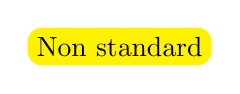
\begin{tikzpicture}
						\node [fill=yellow, rounded corners=5pt] {Non standard};
					\end{tikzpicture}} {undef}
			}
		}
	}
}

\newcommand{\makeProcessTable}[5]{
	%\setcounter{SubProcessStep}{0}
	%\addtocounter{TopProcessStep}{1}
	%\newpage
	%\section{#1}
	\begin{center}
	\fbox{\begin{minipage}{\textwidth}
		\centering
		\begin{tikzpicture}[node distance = 3cm, auto, thick, scale=0.7, every node/.style={transform shape}]
			\input{#2}
		\end{tikzpicture}\\
		\textbf{Mask: #3}
	\end{minipage}}

	\begin{tabular}{|>{\Strut[-0.5]{\rowHeight}}r|}
		\hline
		\textbf{Wafer Cleanliness} \\
		#4
		\hline
        \end{tabular}
	\hspace{0.25cm}
        \begin{tabular}{
			|>{\Strut[-0.5]{\rowHeight}}r
			|C{8.0cm}
			|C{2.0cm}
			|C{3.0cm}
			|C{6.0cm}
			|C{9.0cm}
			|}
		\hline
		\textbf{Step Number} &
		\textbf{Equipment} &
		\textbf{Location} &
		\textbf{Cleanliness} &
		\textbf{Process} &
		\textbf{Requirements} \\
		#5
		\hline
	\end{tabular}
	\end{center}
}

\newcommand{\addProcessStep}[5]{
	\hline
	\addtocounter{SubProcessStep}{1}
	\arabic{TopProcessStep}.\arabic{SubProcessStep} &
	#1 &
	#2 &
	\getWaferCleaninessSymbol{#3} &
	#4 &
	#5
	\\
}

\newcommand{\addLevelCell}[1]{
	\hline
	\getWaferCleaninessSymbol{#1}
	\\
}

\author{David Lanzendörfer}
\title{LibreSilicon process HKUST (NFF)}
\begin{document}
\maketitle
\begin{abstract}
	Copyright © 2017 LANCEVILLE TECHNOLOGY GROUP CO., LIMITED. All rights reserved. \\

This process is licensed under the Libre Silicon public license; you can redistribute it and/or modify it under the terms of the Libre Silicon public license
as published by the Libre Silicon alliance, either version 1 of the License, or (at your option) any later version.

This design is distributed in the hope that it will be useful, but WITHOUT ANY WARRANTY; without even the implied warranty of MERCHANTABILITY or FITNESS FOR A PARTICULAR PURPOSE.
See the Libre Silicon Public License for more details. \\

This document is part of the specification of the free silicon manufacturing standard for manufacturing the LibreSilicon standard logic cells\footnote{\url{https://git.libresilicon.com/?p=redmine/standard-cell-lib.git;a=summary}} and related free technology nodes from the LibreSilicon project.

For this initial revision 0.1 a gate-first approach has been chosen which led to the choice of polysilicon as the gate electrode material because of the simplicity of the gate alignment.
For better isolation properties of the transistors and gates in overall a box-isolation approach has been chosen.
All of these choices have been made with the future scale down from the recent $1 \mu m$ to smaller structure sizes.
\textbf{This process is for manufacturing $1 \mu m$ only!}
But further releases which will have been tested with smaller structure sizes can be expected.
 \\
	Please see the document with the generic steps\footnote{\url{https://github.com/libresilicon/process/raw/master/process_steps/process_hightech/process_hightech_steps.pdf}}
	in order to get a detailed description of the different steps.	
\end{abstract}
\vfill
\newpage

Process Flow of Lanceville Technologies LibreSilicon 1\um 

\begin{itemize}
	\item Project: LibreSilicon 1\um
	\item Name: Lanceville Technologies Group
	\item Substrate: P-Substrate silicon wafer <100>
	\item Date: \today
\end{itemize}

\begin{mdframed}[linewidth=2pt,linecolor=black]
\begin{center}
	\begin{tikzpicture}[node distance = 3cm, auto, thick,scale=0.65, every node/.style={transform shape}]
		\fill[isolationoxide] (0.0,\LowerMoreMetalTwo) rectangle (55.0,\UpperGlass);

\fill[isolationoxide] (0.0,\LowerMoreMetal) rectangle (55.0,\LowerMoreMetalTwo);

\input{tikz_process_steps/metal2.a.tex}

\paintscaledvias{white}{\UpperMoreMetal}{\LowerMoreMetalTwo}{0}


\fill[nitride] (0,\LowerMoreMetalTwo) rectangle (55,\LowerMoreMetalTwo+0.5);
\fill[isolationoxide] (0,\LowerMoreMetalTwo) rectangle (55,\LowerMoreMetalTwo+0.25);

\paintscaledvias{nitride}{\LowerMoreMetalTwo+0.25}{\UpperMoreMetalTwo+0.5}{1.00}
\paintscaledvias{isolationoxide}{\LowerMoreMetalTwo}{\UpperMoreMetalTwo+0.25}{0.75}

\paintscaledvias{gray}{\UpperMoreMetal}{\LowerMoreMetalTwo}{0.25}
\paintscaledvias{gray}{\LowerMoreMetalTwo}{\UpperMoreMetalTwo}{0.50}

\paintscaledvias{brown}{\UpperMoreMetal+0.25}{\LowerMoreMetalTwo+0.3}{-0.1}
\paintscaledvias{brown}{\LowerMoreMetalTwo+0.3}{\UpperMoreMetalTwo}{0.5}


\paintscaledvias{white}{\UpperMoreMetalTwo}{\UpperGlass}{0.25}

		\node at (5,-0.5) {\textbf{\huge{PMOS}}};
		\node at (13,-0.5) {\textbf{\huge{NMOS}}};
		\node at (22,-0.5) {\textbf{\huge{SONOS flash cell (PMOS)}}};
		\node at (30,-0.5) {\textbf{\huge{NPN BJT}}};
		\node at (38,-0.5) {\textbf{\huge{PNP BJT}}};
		\node at (46,-0.5) {\textbf{\huge{Polysilicon diode}}};
		\node at (52,-0.5) {\textbf{\huge{Polyresistor}}};
	\end{tikzpicture}
\end{center}
\end{mdframed}
\newpage
\input{\inctable}
\newpage
\centering
\includegraphics[width=0.75\textwidth]{apple}
\end{document}
